\section{Analyse post-mortem}
    \subsection{Technologies}
        \subsubsection{Kotlin}
        L'utilisation de Kotlin a été un énorme point positif. En effet, la syntaxe simplifié de celui-ci a généré un développement plus rapide, du code plus facile à lire et un code plus facile à maintenir. Par exemple, les data class de Kotlin permettent d'abstraire en quelques lignes de code des centaines de lignes de Java. De plus, Kotlin est en voie de devenir le langage officiel d'Android, nous étions donc réjouis d'avoir cet occasion d'apprentissage.
        
        \subsubsection{Spring}
        L'utilisation du framework Spring n'a pas été apprécié dans le projet, car il y avait trop de magie et de configurations à faire. De plus, ce framework était trop lourd. Le temps de démarrage était très élevé malgré que notre projet était minuscule comparé à ce qu'un projet avec Spring peut devenir.
        
        En rétrospective, l'équipe aurait dû choisir un framework Kotlin plus simpliste et plus approprié.

        \subsubsection{Gitlab en déploiement continu}
        Gitlab en déploiement continue fût un net positif dans notre équipe. Il était si simple de déployer, car tout était automatisé. En effet, il suffisait de fusionner une branche à Master et Gitlab se chargeait de déployer automatiquement sur les VM de l'université.

        En contrepartie, il a été extrêmement complexe d'instaurer cette automatisation. Cependant, nous pensons que l'effort en valait la peine à cause de l'utilisation intensive que nous en avons fait.
        
        \subsubsection{React Native}
        React Native fût un choix controversé dans l'équipe. En effet, celui-ci permet de développer rapidement sur des ordinateurs Windows et Mac pour les plateformes Android et IOS avec un seul codebase de manière native.

        Cependant, React Native est une sorte de dette technique, car éventuellement nous devrions reprogrammer certaines parties de notre application à l'aide des langages natifs si nous voulons atteindre de meilleurs performances et plus de personnalisation.

        Cependant, dans le cadre du projet de session, React Native constituait un avantage net, car notre objectif était de livrer un produit fini avec de plus de fonctionnalités possible en 15 semaines. React Native était le choix parfait pour atteindre les objectifs que nous nous étions fixés.

        \subsubsection{Expo}
        Expo est un outil gratuit et facile d'utilisation qui nous a permis d'accélérer le développement de plusieurs fonctionnalités tel les notifications. De plus, expo nous permet de compiler les applications IOS et Android à l'aide d'une seule commande sur Windows ou Mac sans avoir à installer des toolchains sur les machines de développement. Expo fût très apprécié par l'équipe et serait à réutiliser si nous refaisions un projet similaire.
        
    \subsection{Gestion}
    Au début du projet nous utilisions Gitlab pour faire la gestion de projet. Cependant, après 30 jours, la version d'essais a expiré et nous nous sommes aperçu bien vite que les fonctionnalités payantes étaient plus que nécessaire pour un bonne gestion de projet.

    Vu le prix démesuré de Gitlab, nous avons exploré les alternatives et notre choix s'est arrêté sur JIRA. Celui-ci coûtait 13\$ par mois pour toute l'équipe et nous avons découvert un logiciel qui était bien meilleur que Gitlab.

    Notre expérience avec JIRA a été si positive que nous serions prêt à le réutiliser pour notre projet de fin de baccalauréat ou à le recommander en entreprise.

    \begin{figure}[hp] \centering
        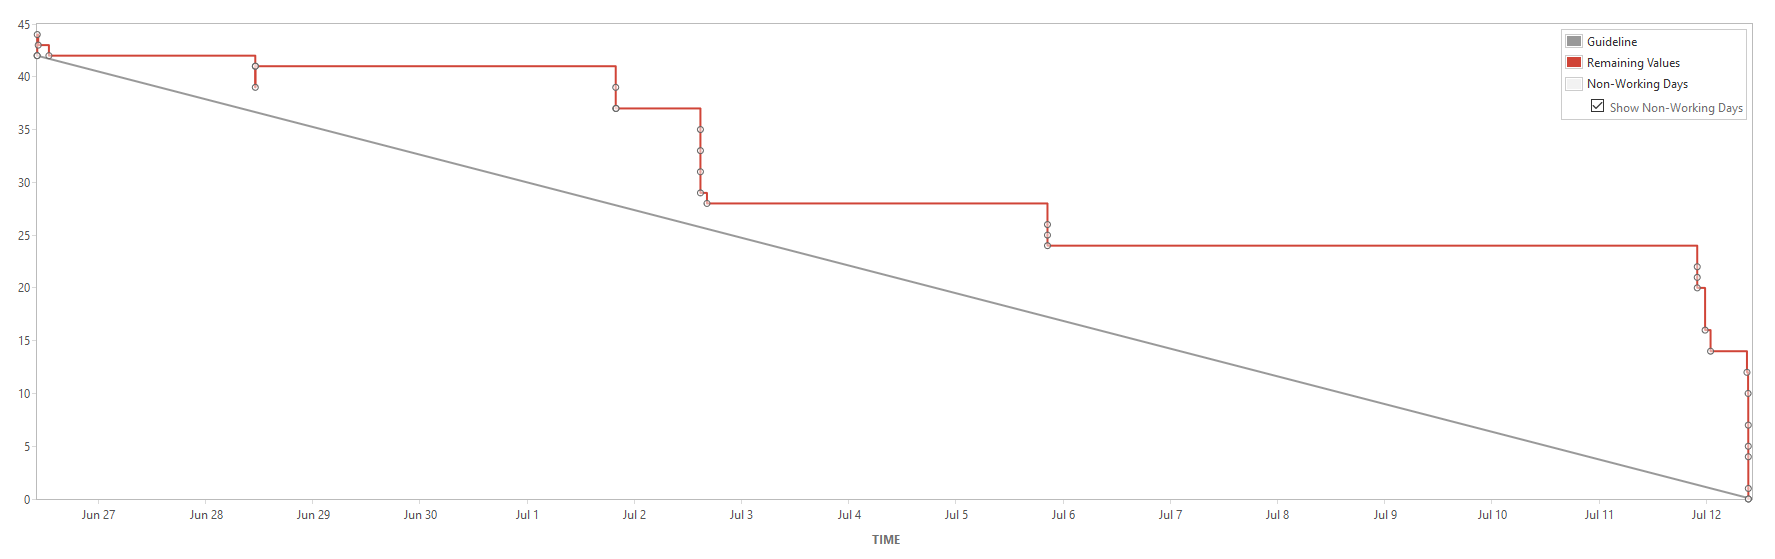
\includegraphics[width=\textwidth]{Figures/burndown}
        \caption{Burndown Chart du troisième sprint du projet}
        \label{fig.burndown}
    \end{figure}

    Ci-dessus nous pouvons voir le burndown chart du troisième sprint. Nous pouvons voir que le principal problème rencontré par l'équipe a été que nous ne mettions pas toujours à jour le statut de de nos tâches. Ainsi, lors des réunions, nous avions tendance à fermer beaucoup de tâche d'un coup. On peut aussi remarquer que l'équipe avait parfois de la difficulté à faire avancer le projet en même temps que certains APP plus demandant (APP3 et APP4 notamment). Une division en plus petites tâches et un suivi plus serré devrait régler ces problèmes lors de nos projets futurs.

    \subsection{Travail d'équipe et cohésion}
    Le travail d'équipe s'est bien passé tout au long du projet. Dû à la grande différences entre les technologies utilisés dans le projet, nous avons commencé à chacun se spécialiser dans un aspect. Par exemple, certain membres de l'équipe s'occupaient des fonctionnalités mobiles en javascript tandis que d'autre faisaient les fonctionnalités du serveur en Kotlin. De plus, même au sein des équipe mobile et backend il y avait des spécialités. Par exemple, au sien de l'équipe mobile il y avait une personne qui était spécialiste des détails de UI.

    Ensuite, l'équipe possédait une très bonne cohésion. En effet, malgré les différents niveaux de compétences, les membres ont travaillé ensemble pour que tout le monde atteigne le même niveau. Il y a donc eu un grand partage de connaissances.

    Finalement, nous étions très motivé par notre projet, malgré un relâchement en milieu de parcours. En effet, au milieu du projet nous n'avons pas reçu les accès que nous nous étions fait promettre en début de session. Cependant, l'équipe a su contourner cet imprévu en trouvant un moyen alternatif d'avoir un produit fini à temps pour la remise. Cet épisode nous a préparé à la vie réel, car souvent sur le marché du travail nous allons faire face à des situation ou des fournisseurs ne livrent pas ce qui était attendu et qu'il faut tout de même livrer un produit fonctionnel.
    